% Documents setup
\documentclass[11pt]{book}

% fix for pandoc 1.14
\providecommand{\tightlist}{%
  \setlength{\itemsep}{0pt}\setlength{\parskip}{0pt}}

\usepackage{tabu} % https://tex.stackexchange.com/questions/50332/vertical-spacing-of-a-table-cell

% Location of the csas-style repository: adjust path as needed
\newcommand{\locRepo}{csas-style}

% Use the style file in the csas-style repository (res-doc.sty)
\usepackage{\locRepo/res-doc}

% header-includes from R markdown entry


% Headers and footers
\lhead{}
% \lhead{}
\rhead{}
% \rfoot{DRAFT - DO NOT CITE}

%%%% Commands for title page etc %%%%%

% Publication year
\newcommand{\rdYear}{}

% Publication month
\newcommand{\rdMonth}{}

% Report number
\newcommand{\rdNumber}{XXX}

% Region
\newcommand{\rdRegion}{Pacific Region}

% Title
\newcommand{\rdTitle}{}

\newcommand{\rdISBN}{}
\newcommand{\rdCatNo}{}

% Author names separated by commas and ', and' for the last author in the format 'M.H. Grinnell' (use \textsuperscript{n} for addresses)
\newcommand{\rdAuth}{}

% Author names reversed separated by commas in the format 'Grinnell, M.H.'
\newcommand{\rdAuthRev}{}

% Author addresses (use \textsuperscript{n})
\newcommand{\rdAuthAddy}{}

\newcommand{\citationOtherLanguage}{}

% Name of file with abstract and resume (see \abstract in inst/csas-style/res-doc.sty)
\newcommand{\rdAbstract}{\abstract{}}

%%%% End of title page commands %%%%%

% \pdfcompresslevel=5 % faster PNGs

\setcounter{section}{0}

\bibliographystyle{csas-style/res-doc}

\usepackage{amsmath}
\usepackage{bm}

% commands and environments needed by pandoc snippets
% extracted from the output of `pandoc -s`
%% Make R markdown code chunks work
\usepackage{array}
\usepackage{amssymb,amsmath}
\usepackage{color}
\usepackage{fancyvrb}

% From default template:
\newcommand{\VerbBar}{|}
\newcommand{\VERB}{\Verb[commandchars=\\\{\}]}
\DefineVerbatimEnvironment{Highlighting}{Verbatim}{commandchars=\\\{\},formatcom=\color[rgb]{0.00,0.00,0.00}}
\usepackage{framed}
\definecolor{shadecolor}{RGB}{248,248,248}
\newenvironment{Shaded}{\begin{snugshade}}{\end{snugshade}}
\newcommand{\AlertTok}[1]{\textcolor[rgb]{0.94,0.16,0.16}{#1}}
\newcommand{\AnnotationTok}[1]{\textcolor[rgb]{0.56,0.35,0.01}{\textbf{\textit{#1}}}}
\newcommand{\AttributeTok}[1]{\textcolor[rgb]{0.77,0.63,0.00}{#1}}
\newcommand{\BaseNTok}[1]{\textcolor[rgb]{0.00,0.00,0.81}{#1}}
\newcommand{\BuiltInTok}[1]{#1}
\newcommand{\CharTok}[1]{\textcolor[rgb]{0.31,0.60,0.02}{#1}}
\newcommand{\CommentTok}[1]{\textcolor[rgb]{0.56,0.35,0.01}{\textbf{#1}}}
\newcommand{\CommentVarTok}[1]{\textcolor[rgb]{0.56,0.35,0.01}{\textbf{\textit{#1}}}}
\newcommand{\ConstantTok}[1]{\textcolor[rgb]{0.00,0.00,0.00}{#1}}
\newcommand{\ControlFlowTok}[1]{\textcolor[rgb]{0.13,0.29,0.53}{\textit{#1}}}
\newcommand{\DataTypeTok}[1]{\textcolor[rgb]{0.13,0.29,0.53}{#1}}
\newcommand{\DecValTok}[1]{\textcolor[rgb]{0.00,0.00,0.81}{#1}}
\newcommand{\DocumentationTok}[1]{\textcolor[rgb]{0.56,0.35,0.01}{\textbf{\textit{#1}}}}
\newcommand{\ErrorTok}[1]{\textcolor[rgb]{0.64,0.00,0.00}{\textit{#1}}}
\newcommand{\ExtensionTok}[1]{#1}
\newcommand{\FloatTok}[1]{\textcolor[rgb]{0.00,0.00,0.81}{#1}}
\newcommand{\FunctionTok}[1]{\textcolor[rgb]{0.00,0.00,0.00}{#1}}
\newcommand{\ImportTok}[1]{#1}
\newcommand{\InformationTok}[1]{\textcolor[rgb]{0.56,0.35,0.01}{\textbf{\textit{#1}}}}
\newcommand{\KeywordTok}[1]{\textcolor[rgb]{0.13,0.29,0.53}{\textit{#1}}}
\newcommand{\NormalTok}[1]{#1}
\newcommand{\OperatorTok}[1]{\textcolor[rgb]{0.81,0.36,0.00}{\textit{#1}}}
\newcommand{\OtherTok}[1]{\textcolor[rgb]{0.56,0.35,0.01}{#1}}
\newcommand{\PreprocessorTok}[1]{\textcolor[rgb]{0.56,0.35,0.01}{\textbf{#1}}}
\newcommand{\RegionMarkerTok}[1]{#1}
\newcommand{\SpecialCharTok}[1]{\textcolor[rgb]{0.00,0.00,0.00}{#1}}
\newcommand{\SpecialStringTok}[1]{\textcolor[rgb]{0.31,0.60,0.02}{#1}}
\newcommand{\StringTok}[1]{\textcolor[rgb]{0.31,0.60,0.02}{#1}}
\newcommand{\VariableTok}[1]{\textcolor[rgb]{0.00,0.00,0.00}{#1}}
\newcommand{\VerbatimStringTok}[1]{\textcolor[rgb]{0.31,0.60,0.02}{#1}}
\newcommand{\WarningTok}[1]{\textcolor[rgb]{0.56,0.35,0.01}{\textbf{\textit{#1}}}}

\newcommand{\lt}{\ensuremath <}
\newcommand{\gt}{\ensuremath >}

%Defines cslreferences environment
%Required by pandoc 2.8
%Copied from https://github.com/rstudio/rmarkdown/issues/1649
% % \newlength{\cslhangindent}
% \setlength{\cslhangindent}{1.5em}
% \newenvironment{cslreferences}%
%   {}%
%   {\par}
% 
\DeclareGraphicsExtensions{.png,.pdf}
\begin{document}

\frontmatter

\newcommand{\mli}[1]{\mathit{#1}}
\newcommand{\SB}{\mli{SB}}
\newcommand{\BR}{\mli{BR}}
\newcommand{\AVE}{\text{AVE}}

\hypertarget{science-advice}{%
\section*{SCIENCE ADVICE}\label{science-advice}}
\addcontentsline{toc}{section}{SCIENCE ADVICE}

{[}Mandatory. Maximum length 500 words. Include summary bullets of the following factors affecting the stock that are relevant for decision-making. Please refer to the Guidance Document for standardized language and examples, and what to avoid in this section.{]}

\hypertarget{status}{%
\subsection*{Status}\label{status}}
\addcontentsline{toc}{subsection}{Status}

{[}The Strait of Georgia (SOG) major stock assessment region (SAR) is healthy.{]}

TODO: define the term SAR here

\hypertarget{trends}{%
\subsection*{Trends}\label{trends}}
\addcontentsline{toc}{subsection}{Trends}

{[}Mandatory bullet(s){]}

\hypertarget{ecosystem-and-climate-change-considerations}{%
\subsection*{Ecosystem and Climate Change Considerations}\label{ecosystem-and-climate-change-considerations}}
\addcontentsline{toc}{subsection}{Ecosystem and Climate Change Considerations}

{[}Mandatory bullet(s){]}

TODO: include DDM here and mention other (HG) EAFM work

\hypertarget{stock-advice}{%
\subsection*{Stock Advice}\label{stock-advice}}
\addcontentsline{toc}{subsection}{Stock Advice}

{[}Mandatory bullet(s){]}

\hypertarget{other-management-questions-if-applicable-otherwise-do-not-include}{%
\subsection*{Other Management Questions {[}if applicable, otherwise do not include{]}}\label{other-management-questions-if-applicable-otherwise-do-not-include}}
\addcontentsline{toc}{subsection}{Other Management Questions {[}if applicable, otherwise do not include{]}}

{[}Other bullets if applicable{]}

\hypertarget{basis-for-assessment}{%
\section*{BASIS FOR ASSESSMENT}\label{basis-for-assessment}}
\addcontentsline{toc}{section}{BASIS FOR ASSESSMENT}

\hypertarget{assessment-details}{%
\subsection*{Assessment Details}\label{assessment-details}}
\addcontentsline{toc}{subsection}{Assessment Details}

This report presents science advice for the Pacific Herring Strait of Georgia (SoG) stock assessment region (SAR), which is one of the five major and two minor SARs; the other major and minor SARs are presented in REF(2024SR).

SoG Pacific Herring are assessed using a spatially integrated statistical catch at age herring (SISCAH) modelling framework within a management strategy evaluation (MSE) process (DFO 2023a), fitted using spawn survey indices, fishery age composition data, and commercial catches.

For SoG Herring, the SISCAH operating model includes: density dependent mortality (DDM), integrated surface and dive survey data in the index, commercial fishery timing, and a likelihood function with correlated age-compositions.

A weighted operating model is used for the management procedure evaluation, whereby the weighted model represents a range of productivity characterized by the stock recruitment steepness (\(h\)) and the lower limit on natural mortality (\(M_b\)). This approach better represents the uncertainty in stock productivity rather than using a single estimated value of \(h\).

Details of operating model development are described in Appendix A.

Management procedures (MPs) were simulation tested using a 15-year projection period (2024-2038); only MPs that meet the established conservation objective (DFO 2023b) are presented.

\hypertarget{year-assessment-approach-was-approved}{%
\subsubsection*{Year Assessment Approach was Approved}\label{year-assessment-approach-was-approved}}
\addcontentsline{toc}{subsubsection}{Year Assessment Approach was Approved}

2023 S. D. N. Johnson and Rossi (2024).

\hypertarget{assessment-type}{%
\subsubsection*{Assessment Type}\label{assessment-type}}
\addcontentsline{toc}{subsubsection}{Assessment Type}

Full Assessment and MSE process.

\hypertarget{most-recent-assessment-date}{%
\subsubsection*{Most Recent Assessment Date}\label{most-recent-assessment-date}}
\addcontentsline{toc}{subsubsection}{Most Recent Assessment Date}
\begin{enumerate}
\def\labelenumi{\arabic{enumi}.}

\item
  Last Full Assessment: 2024 (this document).
\end{enumerate}
\hypertarget{assessment-approach}{%
\subsubsection*{Assessment Approach}\label{assessment-approach}}
\addcontentsline{toc}{subsubsection}{Assessment Approach}
\begin{enumerate}
\def\labelenumi{\arabic{enumi}.}
\item
  Broad category: Single stock operating model ensemble (full MSE process).
\item
  Specific category: Index-based, statistical catch-at-age model, density dependent time varying natural mortality, and Beverton-Holt stock-recruitment relationship.
\end{enumerate}
This 2024 SISCAH modelling framework (S. D. N. Johnson and Rossi 2024) includes stock status and MP for SoG Herring.

\hypertarget{stock-structure-assumption}{%
\subsection*{Stock Structure Assumption}\label{stock-structure-assumption}}
\addcontentsline{toc}{subsection}{Stock Structure Assumption}

Stock overview information: SoG Herring is one of five major stocks managed in British Columbia. Data collection and assessment focuses on the core spawn timing associated with the main migratory stock. Adult herring are reported in various areas of the Salish Sea during the summer months indicating some level of non-migratory life history, with the largest component of the stock migrating to the west coast to share summer/ fall feeding grounds with the West Coast Vancouver Island herring.

\hypertarget{reference-points}{%
\subsection*{Reference Points}\label{reference-points}}
\addcontentsline{toc}{subsection}{Reference Points}

A suite of biological and fishery reference points are included for SoG Herring. These are: 1. Fractions of unfished biomass, \({SB_0}\) 1. \({MSY}\) 1. Fractions of \(U_{MSY}\)

In 2018, a biological limit reference point (LRP) was defined for Pacific Herring major stocks as \(0.3SB_0\) in 2018, where \({SB_0}\) is the long-term average estimated unfished spawning biomass (Kronlund et al. 2017).

Candidate USRs were first introduced in Cleary et al. (2019) and a formal analysis of USR options was undertaken in 2022 with results presented in DFO (2023b). In 2023, DFO Resource Management selected and implemented a provisional USR of \(\overline{\mathit{SB}}\), implemented as a performance metric within 2022/23 IFMP process.

Add table here. - Limit Reference Point (LRP) - Upper Stock Reference (USR) - Removal Reference (RR): not yet determined - Target (TRP): not yet determined (USR=TRP) - Habitat or Ecosystem Reference Points: included indirectly via DDM (state how)

\hypertarget{fishery-management-objectives}{%
\subsection*{Fishery management objectives}\label{fishery-management-objectives}}
\addcontentsline{toc}{subsection}{Fishery management objectives}

A core set of fisheries management objectives (DFO 2020) were introduced to the Pacific Herring MSE process in 2019. The first of these is a conservation objective, which is centered on the LRP.
\begin{enumerate}
\def\labelenumi{\arabic{enumi}.}
\item
  Maintain spawning biomass at or above the LRP with at least 75\% probability over three Pacific Herring generations (i.e., avoid a biomass limit; \(P(\mathit{SB}_t \geq 0.3 \mathit{SB}_0) \geq 0.75\)),
\item
  Maintain spawning biomass at or above the USR with at least 50\% probability over three Pacific Herring generations (i.e., achieve a target biomass; \(P(\mathit{SB}_t \geq \mathit{SB}_{targ}) \geq 0.50\)),
\item
  Maintain average annual variability (AAV) in catch below 25\% over three Pacific Herring generations (i.e., minimize catch variability; \(\text{AAV} < 0.25\)), and
\item
  Maximize average annual catch over three Pacific Herring generations (i.e., maximize average catch).
\end{enumerate}
Operating model development began for Herring MSE in 2015, however a fully specified set of objectives has not yet been developed for each SAR. DFO will continue to collaborate with coastal First Nations to develop area-specific objectives FSC fisheries as well as SOK fisheries (where applicable). In addition, DFO will continue to engage with the herring industry and government and non-government organizations to describe broader objectives related to conservation, economics, and access.

\hypertarget{stock-status}{%
\subsection*{Stock Status}\label{stock-status}}
\addcontentsline{toc}{subsection}{Stock Status}

SoG stock status is defined from the operating model (Appendix A).

\hypertarget{harvest-decision-rule}{%
\subsection*{Harvest Decision Rule}\label{harvest-decision-rule}}
\addcontentsline{toc}{subsection}{Harvest Decision Rule}

{[}Optional (otherwise, do not include). Maximum length 100 words.{]} This is defined using the MSE MP evaluations \ldots{}

\hypertarget{data}{%
\subsection*{Data}\label{data}}
\addcontentsline{toc}{subsection}{Data}

There are three types of input data used for the Pacific Herring stock assessment: catch data, biological data, and a fishery independent survey index.

JC: Finish this.

Note that we refer to `year' instead of `herring season' in this report; therefore 2024 refers to the 2023/2024 Pacific Herring season.

\hypertarget{assessment}{%
\section*{ASSESSMENT}\label{assessment}}
\addcontentsline{toc}{section}{ASSESSMENT}
\begin{itemize}

\item
  Example cross-reference: Stock status in relation to four indicators (see Figure~\ref{fig:indicators}).
\end{itemize}
{[}Mandatory panel of images comes first -- example shown. Refer to the Guidance Document for options and further instructions.{]}


\begin{figure}
\centering
\includegraphics{knitr-figs-docx/indicators-1.png}
\caption{\label{fig:indicators}Stock status indicators for Pacific Herring in the Strait of Georgia (SoG) major stock assessment region (SAR) from 1950 to 2022. (A) Catch (line) and total allowable catch (TAC; dashed line). (B) Spawning stock biomass (SSB) in relation to the limit reference point (LRP; dashed red line) and upper stock reference (USR; dotted green line). (C) Fishing mortality (F; black line), removal reference (RR; dashed red line), and natural mortality (M; dotted line). (D) Recruitment of age-2 fish. Legend: lines indicate median values, grey shading indicates 90\% confidence intervals, mortality is per year (yr), biomass is in tonnes (t), and recruitment is number of fish.}
\end{figure}
{[}Optional. Add an additional optional panel of 4 indicators if relevant to developing advice.{]} {[}Optional. If the FSAR or FSRR is being used to provide advice for more than one stock, the mandatory panel can be repeated for each stock.{]}

\hypertarget{historical-and-recent-stock-trajectory-and-trends}{%
\subsection*{Historical and Recent Stock Trajectory and Trends}\label{historical-and-recent-stock-trajectory-and-trends}}
\addcontentsline{toc}{subsection}{Historical and Recent Stock Trajectory and Trends}

{[}Mandatory. Maximum text length one page. Must be first section in Assessment section.{]}

{[}Report trends in relevant indicator(s), one per paragraph, in the following format:{]}

Insert \texttt{stock\_status\_text()} function to automate text:
\begin{itemize}

\item
  Estimated unfished spawning biomass \(\mathit{SB}_0\) is 138,491 t, and the LRP of \(0.3\mathit{SB}_0\) is 41,547 t (posterior medians). Compared to last year, estimated spawning biomass in 2023 \(\mathit{SB}_{2023}\) decreased from 75,523 to 72,782 t (posterior median), and is equivalent to 52.1\% of \(\mathit{SB}_0\) (Tables XX \& XX). Spawning biomass in 2023 is estimated to be above the LRP with a 94.3\% probability (Table XX).
\end{itemize}
\hypertarget{indicator-1-specify-name-e.g.-abundance}{%
\subsubsection*{{[}Indicator 1{]} {[}specify name, e.g., Abundance{]}:}\label{indicator-1-specify-name-e.g.-abundance}}
\addcontentsline{toc}{subsubsection}{{[}Indicator 1{]} {[}specify name, e.g., Abundance{]}:}

{[}Provide values and trends for the stock (as applicable).{]}

\hypertarget{unknown}{%
\subsubsection*{Unknown}\label{unknown}}
\addcontentsline{toc}{subsubsection}{Unknown}

{[}Optional. Indicate what indicators are not available for the stock (as applicable); otherwise, do not include.{]}

\hypertarget{history-of-management-landingsharvesteffort-tac-catch-advice}{%
\subsection*{History of {[}Management; Landings/Harvest/Effort, TAC \& Catch Advice{]}}\label{history-of-management-landingsharvesteffort-tac-catch-advice}}
\addcontentsline{toc}{subsection}{History of {[}Management; Landings/Harvest/Effort, TAC \& Catch Advice{]}}

{[}Mandatory. Title can vary. Maximum text length one page.{]}

Harvest options for 2025 reflect application of simulation-tested MPs for each major SAR, derived from the Herring OM (Benson et al. 2022). OM conditioning was updated in 2022 using historic stock and fishery data from 1950 to 2021; no MP updates were conducted for 2023. MPs are not provided for HG because this is now conducted within the HG rebuilding plan process.\footnote{Haida Gwaii 'íináang \textbar{} iinang Pacific Herring: An ecosystem overview and ecosystem-based rebuilding plan. Draft consultation period occurred September 26 to December 16, 2022; Final approval scheduled for fall 2023.}

\hypertarget{projections-optional-titles-simulations-future-scenarios}{%
\subsection*{Projections {[}optional titles: Simulations, Future Scenarios{]}}\label{projections-optional-titles-simulations-future-scenarios}}
\addcontentsline{toc}{subsection}{Projections {[}optional titles: Simulations, Future Scenarios{]}}

{[}Mandatory. Title can vary. Tables or figures can be used as necessary to support decision-making.{]}

Insert \texttt{proj\_biomass\_text()} function to automate text:
\begin{itemize}

\item
  In the absence of fishing, spawning biomass in 2024 \(\mathit{SB}_{2024}\) is forecast to be 73,375 t (posterior median; Table XX). Spawning biomass in 2024 is forecast to be below the LRP of \(0.3\mathit{SB}_0\) (41,547 t) with a 8.0\% probability, in the absence of fishing (Table XX and Figure XX).
\end{itemize}
\hypertarget{ecosystem-and-climate-change-considerations-1}{%
\subsection*{Ecosystem and Climate Change Considerations}\label{ecosystem-and-climate-change-considerations-1}}
\addcontentsline{toc}{subsection}{Ecosystem and Climate Change Considerations}

Density dependence, where increased mortality is associated with smaller biomass models ecosystem effects such as the increased percentage of natural mortality in the event of lower bio-masses due to a constant predatory removal.

\hypertarget{harvest-decision-rule-outputs}{%
\subsection*{Harvest Decision Rule Outputs}\label{harvest-decision-rule-outputs}}
\addcontentsline{toc}{subsection}{Harvest Decision Rule Outputs}

{[}If applicable (otherwise, do not include).{]}

\hypertarget{evaluation-of-exceptional-circumstancesassessment-triggers}{%
\subsection*{Evaluation of Exceptional Circumstances/Assessment Triggers}\label{evaluation-of-exceptional-circumstancesassessment-triggers}}
\addcontentsline{toc}{subsection}{Evaluation of Exceptional Circumstances/Assessment Triggers}

{[}If applicable (otherwise, do not include).{]}

\hypertarget{bycatch}{%
\section*{BYCATCH}\label{bycatch}}
\addcontentsline{toc}{section}{BYCATCH}

Some fisheries and aquaculture activities in BC cause incidental mortality to Pacific Herring. Similar to SOK harvest as well as FSC and recreational catch, incidental mortality is currently only indirectly accounted for in Pacific Herring stock assessment by estimating annual rates of natural mortality, and is considered minor relative to commercial harvest.

\hypertarget{procedure-for-interim-year-updates}{%
\section*{PROCEDURE FOR INTERIM YEAR UPDATES}\label{procedure-for-interim-year-updates}}
\addcontentsline{toc}{section}{PROCEDURE FOR INTERIM YEAR UPDATES}

{[}Optional (otherwise, do not include).{]}

\hypertarget{other-management-questions}{%
\section*{OTHER MANAGEMENT QUESTIONS}\label{other-management-questions}}
\addcontentsline{toc}{section}{OTHER MANAGEMENT QUESTIONS}

{[}Optional (otherwise, do not include).{]}

\hypertarget{sources-of-uncertainty}{%
\section*{SOURCES OF UNCERTAINTY}\label{sources-of-uncertainty}}
\addcontentsline{toc}{section}{SOURCES OF UNCERTAINTY}

{[}Mandatory. Maximum length 500 words.{]}

\hypertarget{research-recommendations}{%
\subsection*{Research Recommendations}\label{research-recommendations}}
\addcontentsline{toc}{subsection}{Research Recommendations}

{[}Optional (otherwise, do not include).{]}

\hypertarget{list-of-meeting-participants}{%
\section*{LIST OF MEETING PARTICIPANTS}\label{list-of-meeting-participants}}
\addcontentsline{toc}{section}{LIST OF MEETING PARTICIPANTS}

{[}Mandatory. The list is to include the name of each participant and their affiliation.{]}

\hypertarget{sources-of-information}{%
\section*{SOURCES OF INFORMATION}\label{sources-of-information}}
\addcontentsline{toc}{section}{SOURCES OF INFORMATION}

\clearpage

\Appendices


\clearpage

\refstepcounter{chapter}
\label{app:a}
\starredchapter{APPENDIX~\thechapter. APPENDIX A}

This appendix summarises closed loop simulations evaluating candidate management procedures for the Strait of Georgia (SOG) herring fishery. SOG herring is the first BC herring fishery to use the new herring operating model framework, named the Spatially Integrated Statistical Catch-at-Age Herring Operating Model (SISCAH-OM). Although there are several differences between SISCAH and the previous herring assessment and operating models, the main difference in SISCAH-OM is the ability to model density dependent mortality (DDM), where natural mortality is higher when biomass is lower (S. D. N. Johnson and Rossi 2024).

All candidate MPs are tested against a suite of five SISCAH operating models, which incorporate uncertainty in future productivity at both low and high stock sizes. We first summarise the simulation approach, and then present results weighted over the five operating models, with some brief discussion of the management implications.


\clearpage

\refstepcounter{chapter}
\hypertarget{simulation-approach}{%
\starredchapter{APPENDIX~\thechapter. Simulation approach}\label{simulation-approach}}

\newcounter{appendix_2_counter}
\refstepcounter{appendix_2_counter}
\hypertarget{operating-models}{%
\appsection{Operating models}\label{operating-models}}

We define five SOG Herring operating models that test against uncertainty in productivity at high and low stock sizes. Productivity at high stock sizes is influenced by the \(M_b\) parameter, which represents the average mortality rate at very high biomass (generally above unfished levels). At low stock size, productivity is more influenced by the stock-recruit relationship's steepness parameter \(h\), which is the ratio of recruitment at 20\% of unfished to the unfished recruitment \(R_0\). Overall \(h\) is better estimated for stocks where the history includes recovery from very low stock sizes. Since this isn't case for SOG, we capture some of the uncertainty around \(M_b\) and \(h\) by considering operating models with different values for those parameters. First we used an established value of \(h=0.70\) (\textbf{cleary2019?}) and ran the operating model with a suite of \(M_b\) values, examined the likelihood profiles and determined that \(M_b=0.562\) produced the lowest negative-log-likelihood. We then ran operating models with \(h\) values of 0.65 and 0.75, while keeping \(M_b=0.562\). Finally to round it out we considered models where \(h=0.70\) and \(M_b\) was 0.532 and 0.584 which correspond to values with equal likelihood values on either side of 0.562 (Figure~\ref{fig:LPfig}).

This creates a cross design (Table~\ref{tab:parRefPtsTable}) with a central OM (called OM1, \(M_b=0.562\) and \(h = 0.7\)) which we gave a weight of 0.34. The remaining operating models are weighted equally\\
with a weight of 0.165.

For all operating models, we report leading OM parameters, current biomass and stock status, and \(MSY\) based reference points (Table~\ref{tab:parRefPtsTable}).
\begin{table}[!h]
\centering
\caption{\label{tab:parRefPtsTable}SISCAH-OM life-history and management parameter values for stock-recruit steepness ($h$), asymptotic lower limit on depensatory $M$ ($M_b$, /yr), unfished biomass ($SB_0$, kt), unfished recruitment ($R_0$, 1e6), unfished mortality ($M_0$, /yr), mortality depensation rate ($m_1$), time-averaged mortality ($\overline{M}$, /yr), surface survey design catchability ($q_s$), spawning biomass in 2023 ($SB_{2023}/SB_0$), stock status ($P(SB_{2023} > 0.3 SB_0)$), spawning biomass at maximum sustainable yield ($SB_{MSY}$, kt), harvest rate targeting maximum sustainable yield ($U_{MSY}$), maximum sustainable yield ($MSY$), upper stock reference ($USR$, kt), harvest rate targeting the upper stock reference ($U_{USR}$), equilibrium yield at the upper stock reference ($Y_{USR}$), harvest rate associated with negative production and higher risk of extirpation ($U_{Crash}$). Uncertainty is shown as the 95\% credible interval where estimates could be drawn from posterior samples (indicated by two parenthetical values), or half the interquartile range where estimates were drawn from 200 year simulations (one parenthetical value).}
\centering
\resizebox{\ifdim\width>\linewidth\linewidth\else\width\fi}{!}{
\begin{tabular}[t]{lrrrrr}
\toprule
  & OM1 & OM2 & OM3 & OM4 & OM5\\
\midrule
\cellcolor{gray!10}{$h$} & \cellcolor{gray!10}{0.70} & \cellcolor{gray!10}{0.65} & \cellcolor{gray!10}{0.75} & \cellcolor{gray!10}{0.70} & \cellcolor{gray!10}{0.70}\\
$M_b$ & 0.562 & 0.562 & 0.562 & 0.532 & 0.584\\
\cellcolor{gray!10}{$SB_0$} & \cellcolor{gray!10}{88.58 (36.93)} & \cellcolor{gray!10}{88.25 (40.18)} & \cellcolor{gray!10}{92.51 (37.14)} & \cellcolor{gray!10}{91.54 (42.55)} & \cellcolor{gray!10}{92.05 (36.67)}\\
$R_0$ & 2145.64 (1671.28, 2753.85) & 2150.36 (1677.67, 2750.14) & 2120.51 (1684.48, 2658.85) & 2001.35 (1579.99, 2519.71) & 2263.97 (1777.08, 2874.07)\\
\cellcolor{gray!10}{$M_0$} & \cellcolor{gray!10}{0.58 (0.56, 0.65)} & \cellcolor{gray!10}{0.58 (0.56, 0.66)} & \cellcolor{gray!10}{0.58 (0.56, 0.64)} & \cellcolor{gray!10}{0.57 (0.53, 0.66)} & \cellcolor{gray!10}{0.6 (0.58, 0.66)}\\
\addlinespace
$m_1$ & 4.52 (2.43, 7.42) & 4.58 (2.33, 7.85) & 4.52 (2.52, 7.77) & 3.92 (2.03, 6.78) & 4.84 (2.64, 8.01)\\
\cellcolor{gray!10}{$\overline{M}$} & \cellcolor{gray!10}{0.6 (0.57, 0.63)} & \cellcolor{gray!10}{0.6 (0.57, 0.64)} & \cellcolor{gray!10}{0.6 (0.57, 0.64)} & \cellcolor{gray!10}{0.59 (0.56, 0.63)} & \cellcolor{gray!10}{0.61 (0.58, 0.64)}\\
$q_s$ & 0.7 (0.57, 0.86) & 0.7 (0.56, 0.86) & 0.71 (0.57, 0.85) & 0.72 (0.58, 0.88) & 0.69 (0.55, 0.84)\\
\cellcolor{gray!10}{$SB_{2023}$} & \cellcolor{gray!10}{84.54 (55.46, 122.08)} & \cellcolor{gray!10}{84.35 (56.53, 122.32)} & \cellcolor{gray!10}{84.64 (54.64, 121.94)} & \cellcolor{gray!10}{84.56 (56.45, 119.75)} & \cellcolor{gray!10}{83.36 (54.37, 118.02)}\\
$SB_{2023}/SB_0$ & 0.91 (0.60, 1.32) & 0.96 (0.64, 1.39) & 0.92 (0.60, 1.33) & 0.95 (0.63, 1.35) & 0.91 (0.59, 1.28)\\
\addlinespace
\cellcolor{gray!10}{$P(SB_{2023} > 0.3 SB_0)$} & \cellcolor{gray!10}{1} & \cellcolor{gray!10}{1} & \cellcolor{gray!10}{1} & \cellcolor{gray!10}{1} & \cellcolor{gray!10}{1}\\
$SB_{MSY}$ & 37.81 (13.27) & 44.71 (17.15) & 34.48 (12.89) & 43.68 (18.23) & 36.35 (15.32)\\
\cellcolor{gray!10}{$U_{MSY}$} & \cellcolor{gray!10}{0.185 (0.077)} & \cellcolor{gray!10}{0.122 (0.066)} & \cellcolor{gray!10}{0.261 (0.079)} & \cellcolor{gray!10}{0.145 (0.063)} & \cellcolor{gray!10}{0.229 (0.072)}\\
$MSY$ & 8.876 (6.578) & 6.480 (5.560) & 12.537 (8.005) & 7.626 (6.113) & 11.329 (7.497)\\
\cellcolor{gray!10}{$USR$} & \cellcolor{gray!10}{67.18 (60.08, 75.49)} & \cellcolor{gray!10}{67.37 (60.38, 76.1)} & \cellcolor{gray!10}{67.46 (60.7, 75.8)} & \cellcolor{gray!10}{66.29 (59.15, 75.4)} & \cellcolor{gray!10}{68.4 (61.21, 77.83)}\\
\addlinespace
$U_{USR}$ & 0.078 (0.102) & 0.060 (0.084) & 0.099 (0.123) & 0.077 (0.098) & 0.096 (0.117)\\
\cellcolor{gray!10}{$Y_{USR}$} & \cellcolor{gray!10}{5.774 (7.848)} & \cellcolor{gray!10}{4.390 (6.444)} & \cellcolor{gray!10}{7.511 (10.040)} & \cellcolor{gray!10}{5.627 (7.455)} & \cellcolor{gray!10}{7.402 (9.393)}\\
$U_{Crash}$ & 0.279 (0.097) & 0.166 (0.115) & 0.419 (0.095) & 0.261 (0.074) & 0.316 (0.112)\\
\bottomrule
\end{tabular}}
\end{table}
\begin{figure}
\pdftooltip{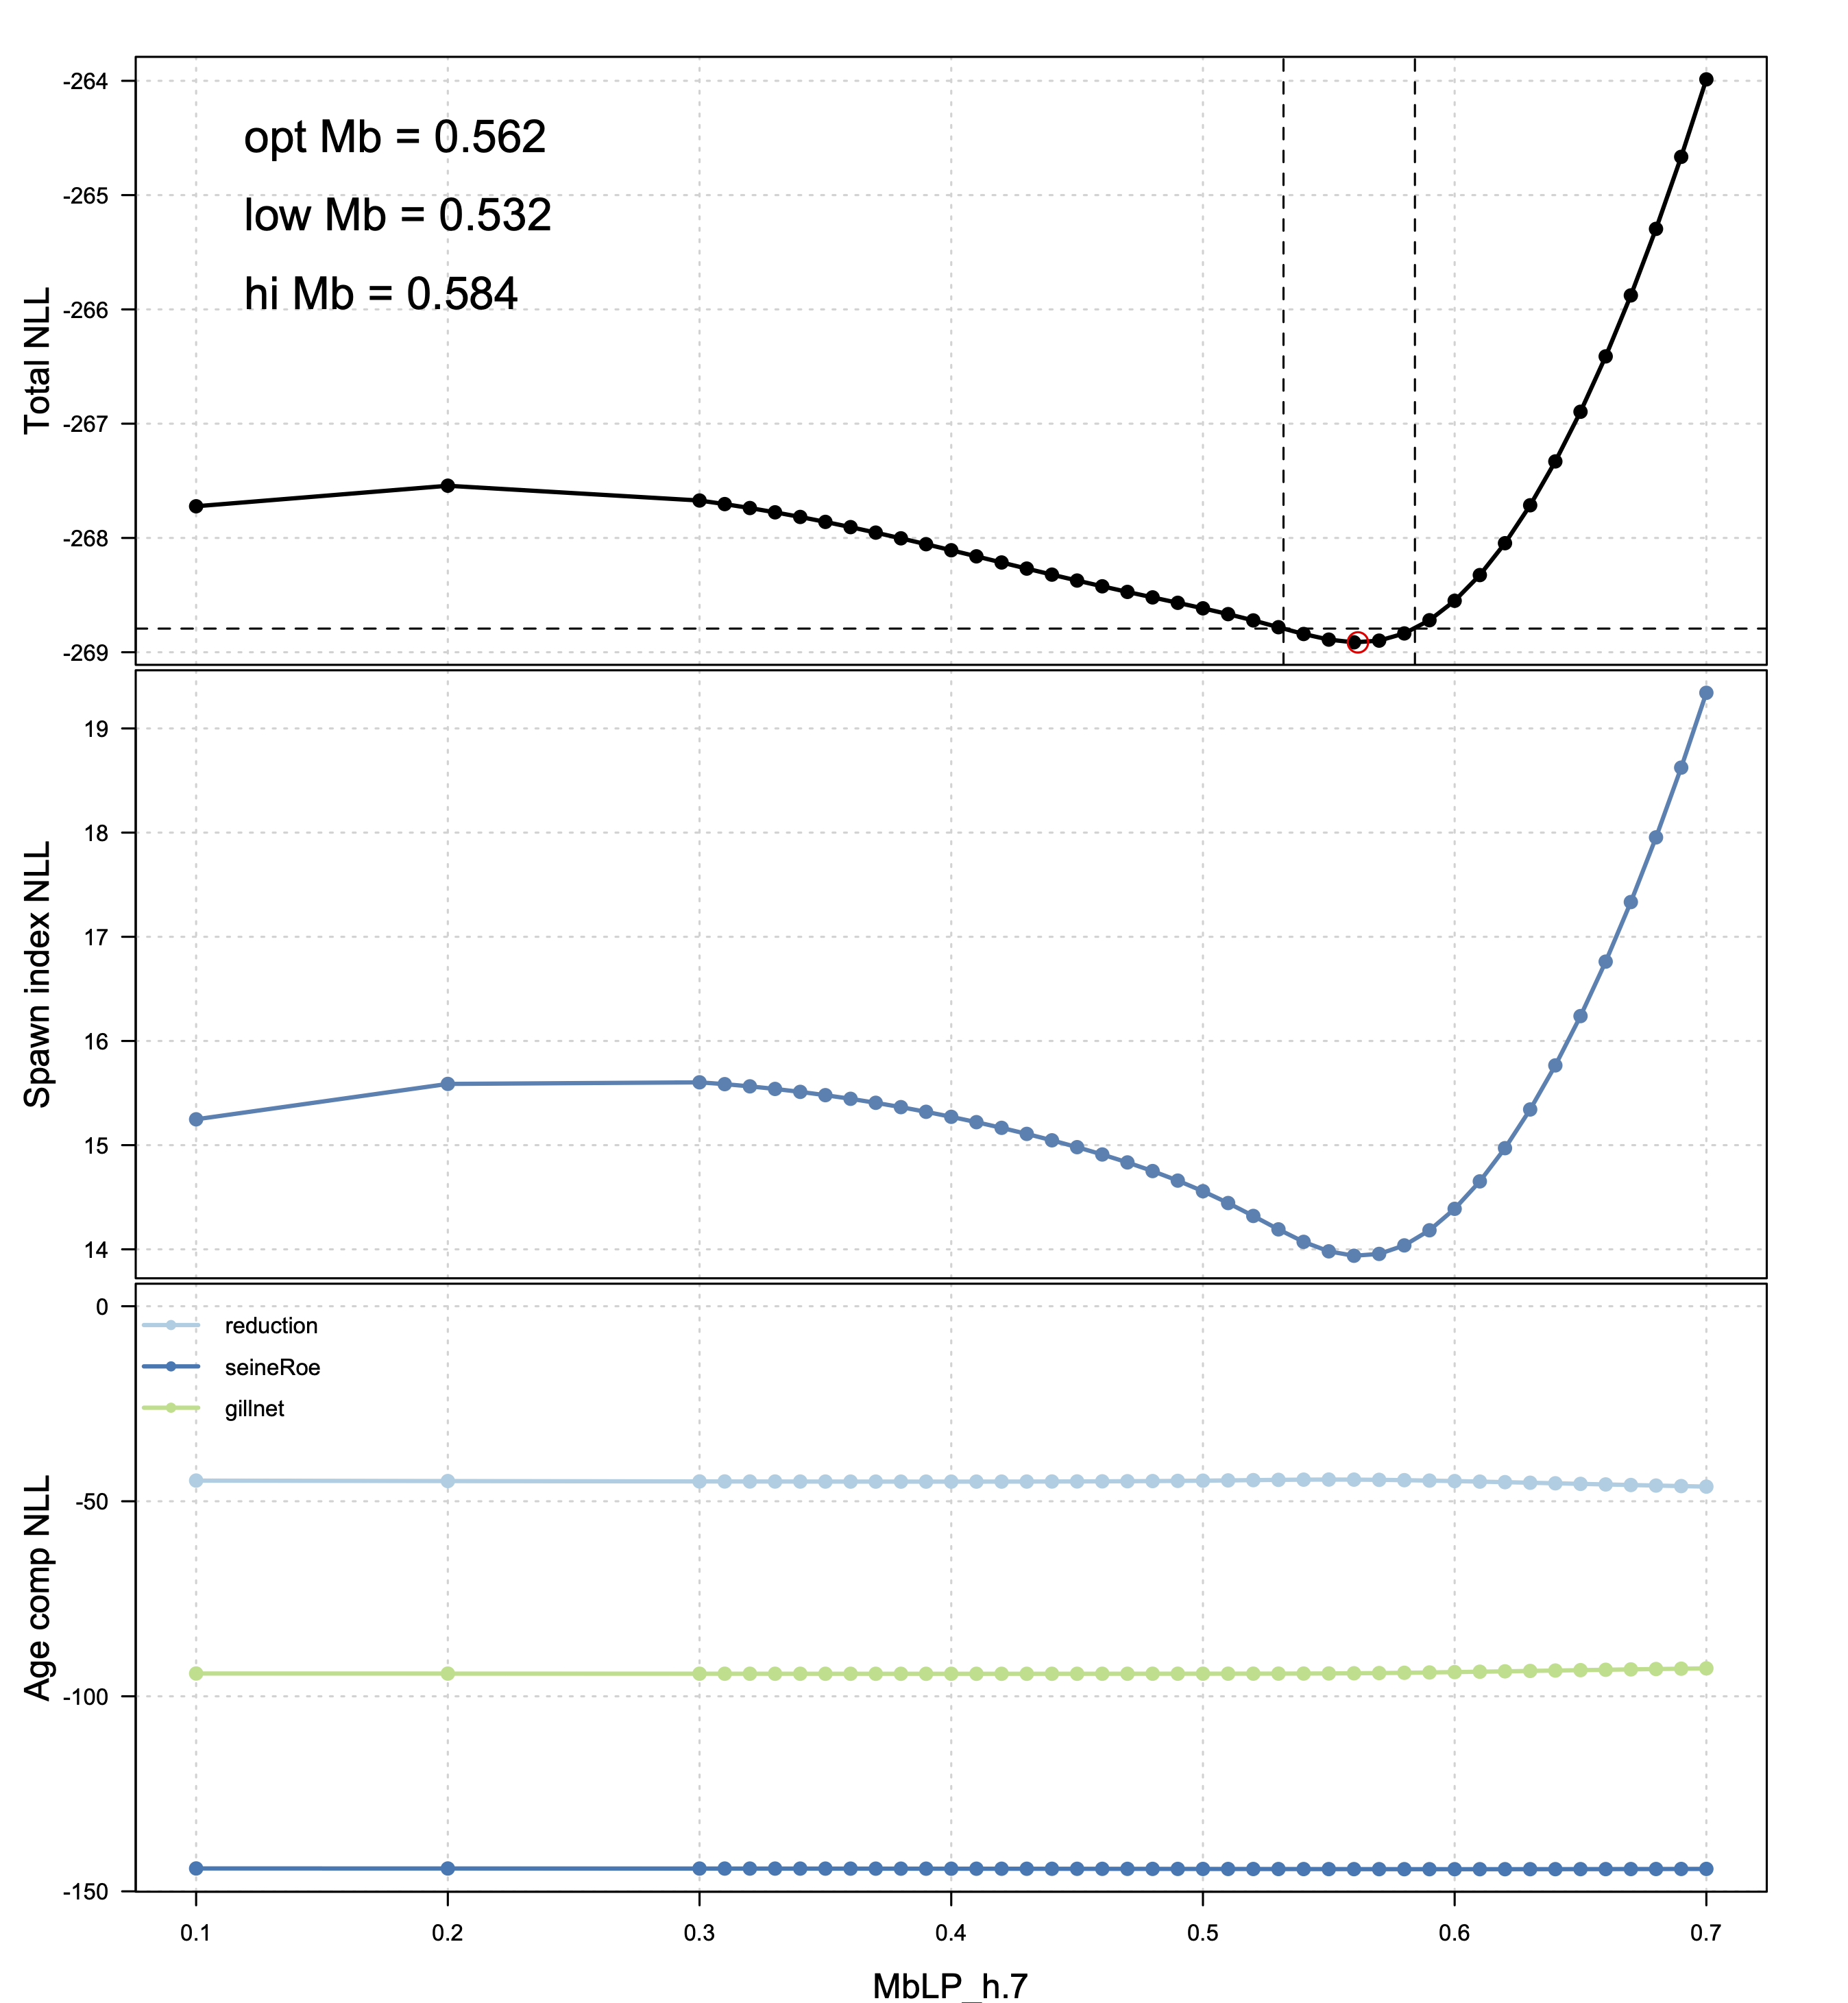
\includegraphics[width=14.98in]{figure/LP_chooseMb}}{Figure} \caption{Fishery monitoring data likelihood function profiles relative to a range of natural mortality asymptotic lower limit ($M_b$) parameter values. The red point shows the most likely value, while the two vertical dashed lines show two values with equal likelihood chosen to bound the central OM1. All SISCAH model fits here have a steepness value of $h = 0.7$}\label{fig:LPfig}
\end{figure}
\hypertarget{management-procedures}{%
\appsection{Management Procedures}\label{management-procedures}}

Management procedures are a combination of data, biomass estimation method (EM), and a harvest control rule (HCR).

All MPs tested here use the same data. The EM, which is fit to those data, is a SISCAH model with a density independent \(M\) (DIM) hypothesis (\textbf{ref?}), which uses a simple random walk to estimate time-varying \(M\). The DIM hypothesis is similar to the previous model used for herring assessments and setting TACs, which used a spline instead of a simple random walk for estimating time-varying \(M\). The EM provides annual estimates of unfished biomass and a 1-year ahead forecast of spawning biomass.

TACs are derived from EM estimates via the harvest control rule. For SOG herring, we use a ``hockey-stick'' shaped function with control points at 30\% and 60\% of unfished biomass. When spawning biomass is estimated to be below the lower control point, the rule sets harvest rates to zero; when biomass estimates are above the upper control point, the rule sets harvest rates to the maximum target harvest rate, called \(maxTHR\). We show results for maximum target harvest rates of 6\% and 14\% (Figure~\ref{fig:hcrPlot}).
\begin{figure}
\centering
\includegraphics{knitr-figs-docx/hcrPlot-1.png}
\caption{\label{fig:hcrPlot}Two harvest control rules tested for candidate SOG herring MPs, showing maximum target harvest rates \(maxTHR\) of 6\% and 14\%.}
\end{figure}
\hypertarget{performance-metrics}{%
\appsection{Performance metrics}\label{performance-metrics}}

MPs are evaluated against two quantitative management objectives, listed below.
\begin{enumerate}
\def\labelenumi{\arabic{enumi}.}
\item
  \(P(B_t > 0.3 B_0) \geq 0.75\), or \textbf{avoid the limit reference point (LRP) with high probability over three herring generations.}
\item
  \(P(B_t > USR) \geq 0.5\), or \textbf{target the upper stock reference (USR) with neutral probability}.
\end{enumerate}
Objective 1, also known as the conservation objective, must be passed by all herring management procedures. Objective 2 is a target objective related to a recently described provisional \(USR\).

To help fishery managers understand trade-offs among biomass and yield, additional quantitative performance metrics are estimated. These metrics do not have a minimum or target value like objectives, but give greater detail on biomass and yield outcomes of each MP over the 15 year simulation.
\begin{enumerate}
\def\labelenumi{\arabic{enumi}.}
\item
  \(P(B_t > B_{MSY})\): The probability that biomass is above \(B_{MSY}\).
\item
  \(P(U_t > U_{MSY})\): The probability that the effective harvest rate is above \(U_{MSY}\).
\item
  \(P(C_t > 650 t)\): The probability of a viable fishery where catch is greater than 650 tonnes.
\item
  \(C_{5pc}\): Catch risk, measured as the fifth percentile of catch over all years and replicates.
\item
  \(\overline{C}\): Median (over replicates) of the average (over years) total landings.
\item
  \(AAV\): Average annual variation in catch, or the mean percentage difference in catch from year-to-year.
\item
  \(C_{2024}\): The MP's TAC in 2024.
\item
  \(\overline{B_{t}/B_0}\): Average biomass depletion from 2024 - 2038.
\item
  \({B_{2038}/B_0}\): Median biomass depletion in 2038.
\item
  \(B_{2038}\): Median biomass in 2038.
\end{enumerate}
Performance metrics are estimated via closed loop feedback simulations with the following simulation algorithm:
\begin{enumerate}
\def\labelenumi{\arabic{enumi}.}
\item
  For each Operating Model, initialize a pre-conditioned simulation model for the period 1951 -- 2023 based on a random draw from the operating model posterior distribution;
\item
  Project the SOG Herring DDM operating model into the future one year at a time. For each year in the projection, apply the following:
  \begin{enumerate}
  \def\labelenumii{\roman{enumii})}

  \item
    Update the time series of commercial catch, catch-at-age, and blended spawn survey data up to time-step t for the stock assessment component of the MP;
  \item
    Use an assessment model (the Density Independent \(M\) SISCAH model) to produce a 1-year ahead forecast of spawning biomass depletion;
  \item
    Determine the target harvest rate associated with the forecast depletion using the HS 30-60 harvest control rule;
  \item
    Using this target harvest rate calculate the total allowable catch from the 1-year ahead biomass forecast;
  \item
    Update the simulated DDM operating model herring population in the with incoming recruitment from the DDM stock-recruit curve with recruitment process errors; density dependant natural mortality; and fishing mortality corresponding to the total allowable catch in the previous step.
  \item
    Repeat steps 2.i - 2.v until the projection period ends (2038).
  \end{enumerate}
\item
  Repeat steps 1. and 2. 99 more times;
\item
  Calculate quantitative performance statistics across all 100 replicates.
\end{enumerate}

\clearpage

\refstepcounter{chapter}
\hypertarget{discussion}{%
\starredchapter{APPENDIX~\thechapter. Discussion}\label{discussion}}

A fishery that meets Objective 1 could target a 13\% harvest rate with an average yield in the 10 - 11 kt range (Table~\ref{tab:statTable}. If management procedures are also targeting the USR (Objective 2), then harvest rates need to drop to around 7\% (as predicted by the reference point estimates, Table~\ref{tab:parRefPtsTable}), and average catches would be closer to the 6 - 7 kt range. Any harvest rate above 13\%, including \(U_{MSY}\) estimates for every OM, do not meet either fishery objective. As such, meeting both fishery objectives requires accepting that TACs will need to be lower in the future, in contrast to the average of around 20 kt up to 2019.

Harvest rates need to be much lower than \(U_{MSY}\) to avoid the LRP with high probability (75\% or more). This is because the LRP is quite high relative to \(B_{MSY}\) (Table~\ref{tab:parRefPtsTable}, Figure~\ref{fig:simEnv}), roughly around 70\% of \(B_{MSY \vert OM1}\) for OM1. For comparison, the default limit reference point in Canadian fisheries policy is 40\% of \(B_{MSY}\) or some proxy, although this is largely applied to longer lived groundfish species with less variable recruitment and lower predation pressures.

The EM based on the Density Independent \(M\) model appears to overestimate biomass in the 1-year ahead forecast. So called positive assessment errors are reflected in the higher than neutral probability the effective harvest rates exceed the maximum target harvest rate (Table~\ref{tab:statTable}, \(P(U_t > U_{ref})\), Figure~\ref{fig:simEnv}, bottom row). As such, MPs should aim for slightly lower maximum harvest rates than the biomass target implies. For example, reference points imply a harvest rate of around 8\% (weighted over OMs) to achieve the USR target in the long term, but positive assessment errors mean that MPs should target closer to 7\%.

The metrics for the probability of a viable fishery and the 5th percentile of simulated TACs are closely related (Table~\ref{tab:statTable}, \(C_t > 650 t\) and \(C_{5pc}\)). Each shows that increasing harvest rates generally means accepting a higher proportion of years with low catch. Additionally, both metrics appear to show an optimal range of 4\% - 6\% harvest rates where the risk of poor fishing is lowest. The \(C_{5pc}\) column is more informative, however, as it uses absolute landings estimates that have a broader range than the more intangible probability of viable fishing.
\begin{table}[!h]
\centering
\caption{\label{tab:statTable}Performance statistics for the selected harvest rates. Objectives that are passed by an MP are indicated by a bullet. Conservation, Biomass, Overfishing, and Viable Fishery metrics are all in probability units. Catch at Risk 5\%, Average Catch, 2024 Catch and Final Biomass are all in biomass units (kt), and Stock Status is biomass depletion relative to unfished (proportion).}
\centering
\resizebox{\ifdim\width>\linewidth\linewidth\else\width\fi}{!}{
\begin{tabular}[t]{ccccccccccccc}
\toprule
\multicolumn{1}{c}{\textbf{ }} & \multicolumn{1}{c}{\textbf{Conservation}} & \multicolumn{2}{c}{\textbf{Biomass}} & \multicolumn{1}{c}{\textbf{Overfishing}} & \multicolumn{1}{c}{\textbf{Viable Fishery}} & \multicolumn{1}{c}{\textbf{Catch at Risk 5\textbackslash{}\% }} & \multicolumn{1}{c}{\textbf{Average Catch}} & \multicolumn{1}{c}{\textbf{Catch Variability}} & \multicolumn{1}{c}{\textbf{2024 Catch}} & \multicolumn{2}{c}{\textbf{Stock Status}} & \multicolumn{1}{c}{\textbf{Final Biomass}} \\
\cmidrule(l{3pt}r{3pt}){2-2} \cmidrule(l{3pt}r{3pt}){3-4} \cmidrule(l{3pt}r{3pt}){5-5} \cmidrule(l{3pt}r{3pt}){6-6} \cmidrule(l{3pt}r{3pt}){7-7} \cmidrule(l{3pt}r{3pt}){8-8} \cmidrule(l{3pt}r{3pt}){9-9} \cmidrule(l{3pt}r{3pt}){10-10} \cmidrule(l{3pt}r{3pt}){11-12} \cmidrule(l{3pt}r{3pt}){13-13}
MP & $B_t \geq 0.3 B_0$ & $B_t \geq B_{MSY}$ & $B_t \geq USR$ & $U_t \geq U_{MSY}$ & $C_t \geq 650 t$ & $C_{5pc}$ & $\overline{C}$ & $AAV$ & $C_{2024}$ & $\overline{B_{t}/B_0}$ & $B_{2038}/B_0$ & $B_{2038}$\\
\midrule
\cellcolor{gray!10}{maxTHR_0.06} & \cellcolor{gray!10}{$\bullet$} & \cellcolor{gray!10}{0.77} & \cellcolor{gray!10}{$\bullet$} & \cellcolor{gray!10}{0.04} & \cellcolor{gray!10}{0.96} & \cellcolor{gray!10}{1.15} & \cellcolor{gray!10}{5.91} & \cellcolor{gray!10}{22.50} & \cellcolor{gray!10}{5.88} & \cellcolor{gray!10}{0.85} & \cellcolor{gray!10}{0.87} & \cellcolor{gray!10}{78.21}\\
maxTHR_0.14 & $\bullet$ & 0.63 & 0.35 & 0.37 & 0.95 & 0.49 & 11.83 & 29.38 & 13.72 & 0.66 & 0.61 & 55.18\\
\bottomrule
\end{tabular}}
\end{table}
\includegraphics{knitr-figs-docx/simEnv-1.png} \# Exceptional Circumstances

Fishery monitoring data collected since the adoption of the current SOG herring MP does is within expectations. In formal language, there is no indication of exceptional circumstances (Figure~\ref{fig:ECfig}), measured by catch and spawn index values within the expected range of previous closed loop simulations.
\begin{figure}
\pdftooltip{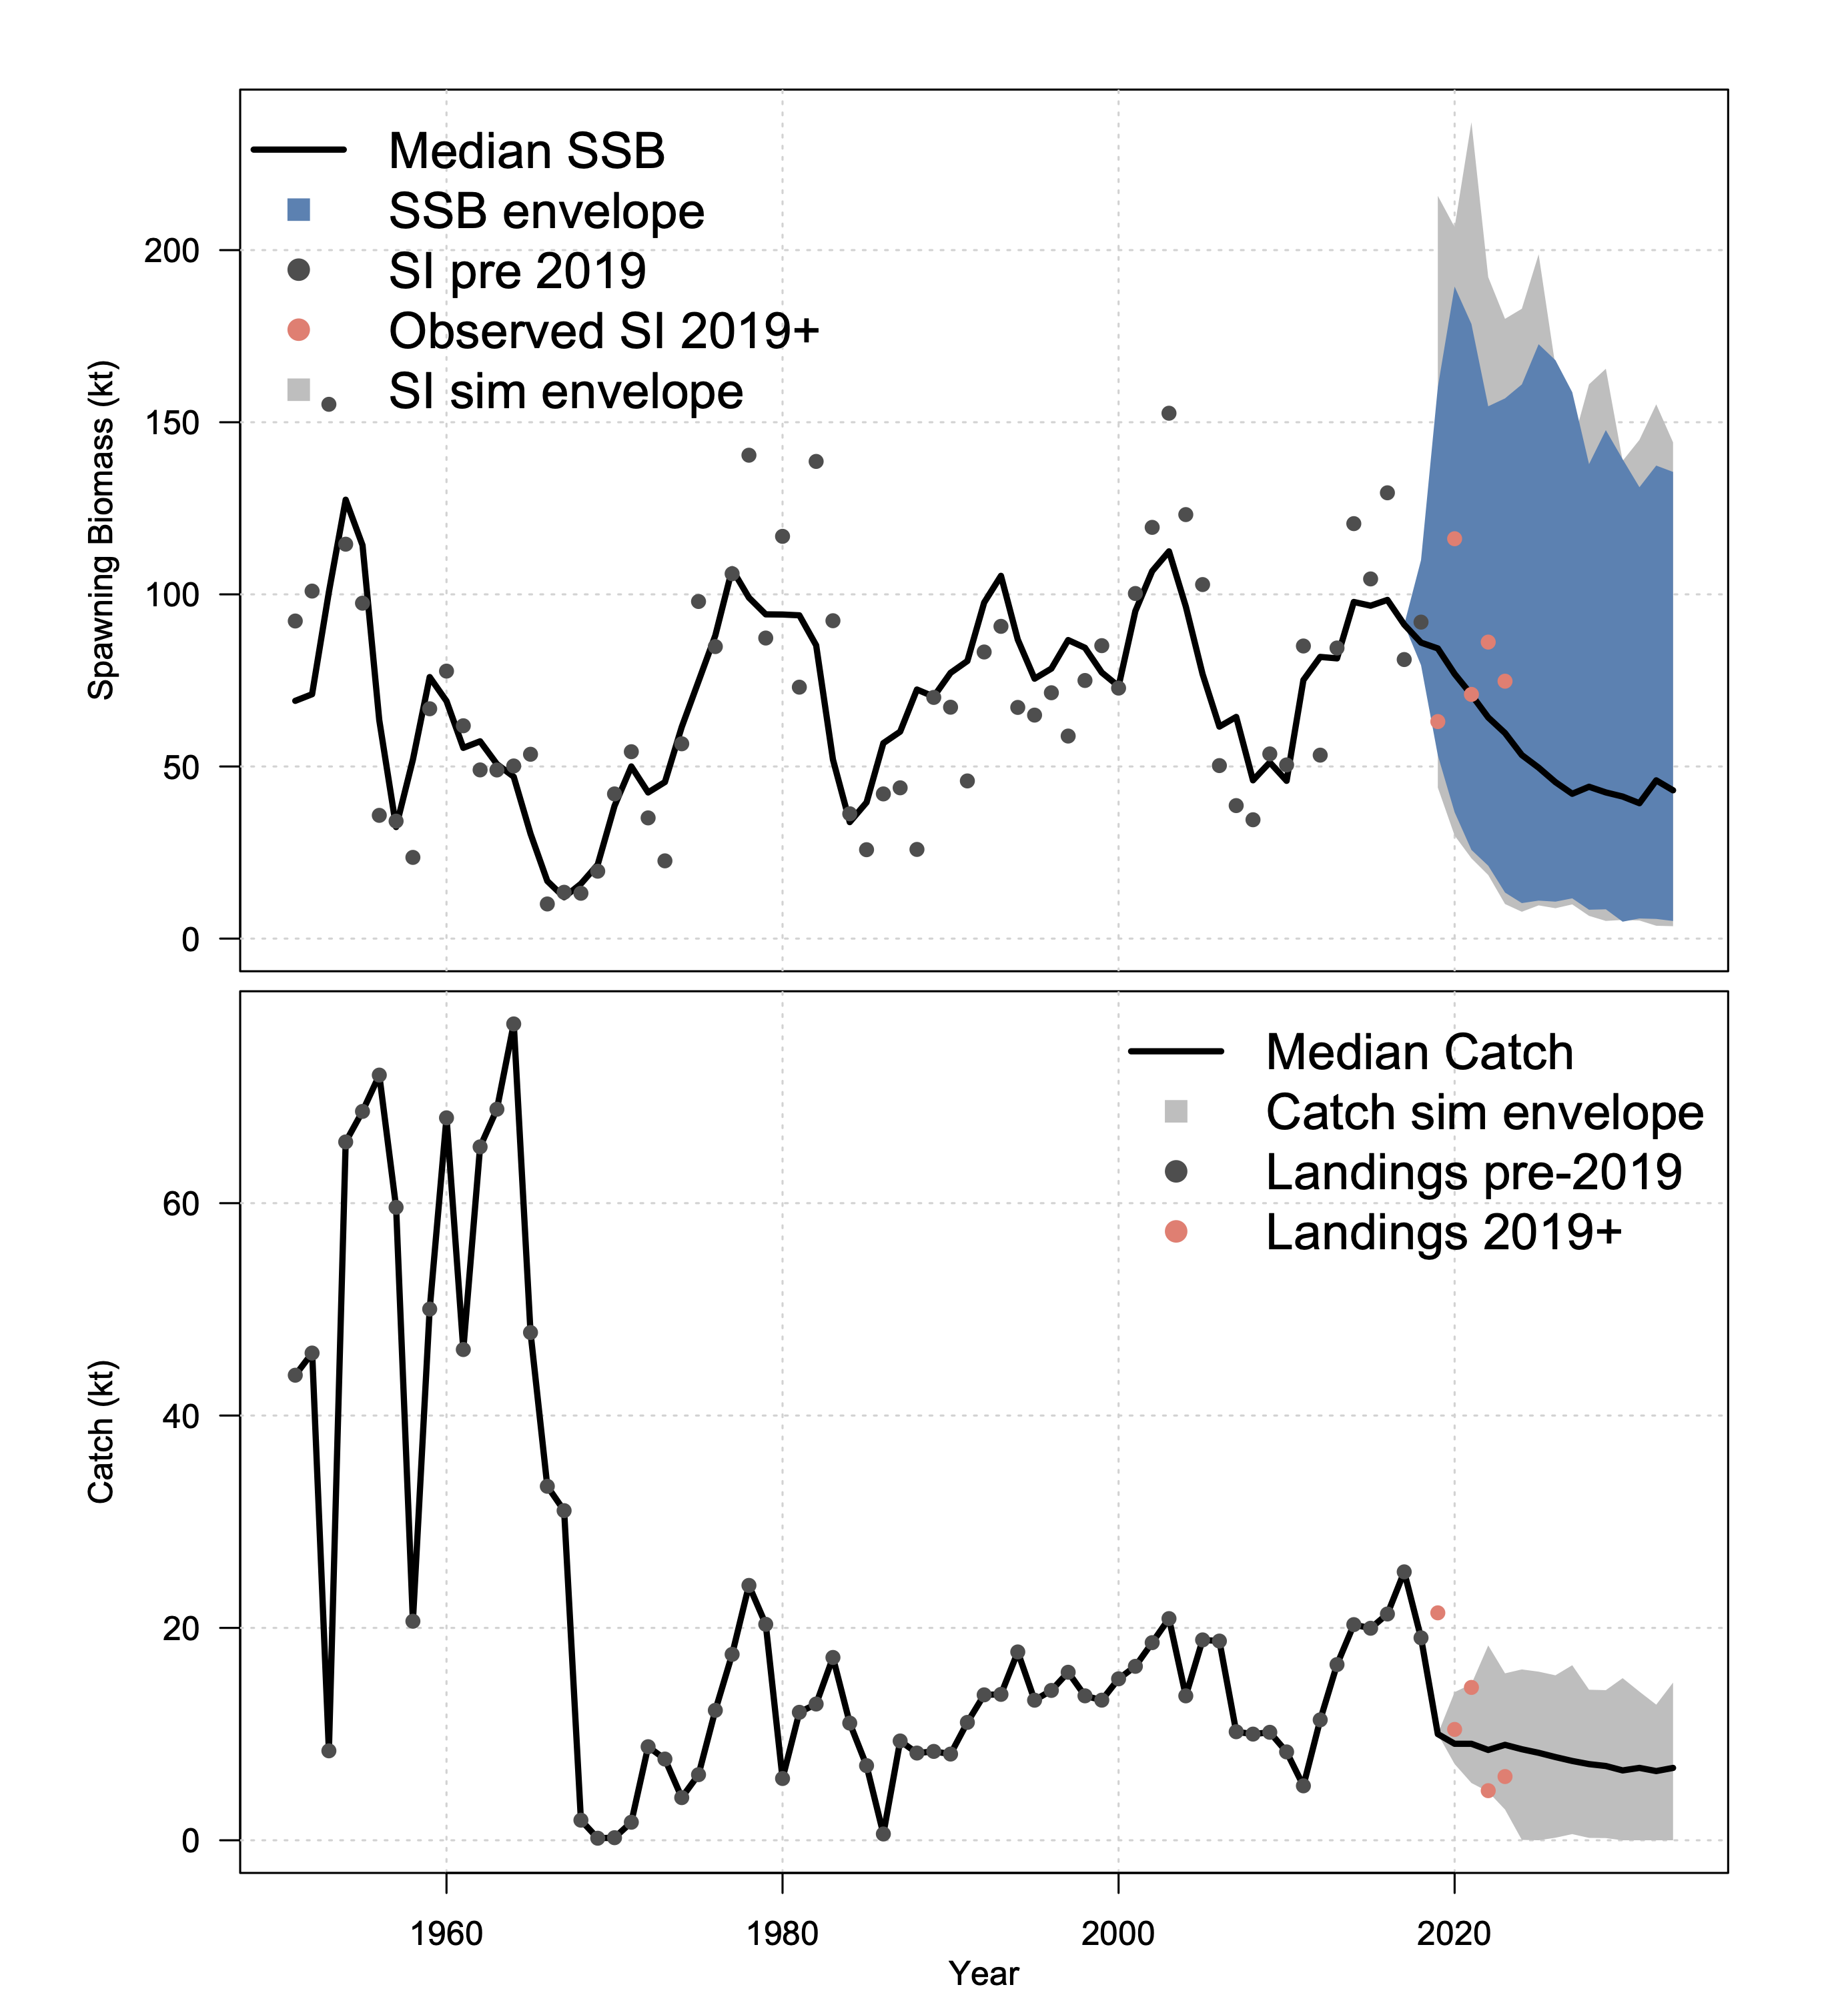
\includegraphics[width=15.39in]{figure/ExceptionalCircumstances}}{Figure} \caption{A graphical test for exceptional circumstances, showing the central 95\% of projected spawn index values (top) and catch values (bottom) using the 2019 SOG operating model, with realised data in the history (black points) and projection (red points) overlaid.}\label{fig:ECfig}
\end{figure}
\hypertarget{refs}{}
\begin{CSLReferences}{1}{0}
\leavevmode{\hypertarget{ref-benson2022}{}}%
Benson, A. J., J. S. Cleary, S. P. Cox, S. Johnson, and M. H. Grinnell. 2022. {``\link{https://www.dfo-mpo.gc.ca/csas-sccs/Publications/ResDocs-DocRech/2022/2022_048-eng.html}{Performance of Management Procedures for {British} {Columbia} {Pacific} {Herring} (\emph{{Clupea} Pallasii}) in the Presence of Model Uncertainty: Closing the Gap Between Precautionary Fisheries Theory and Practice}.''} \emph{DFO Can. Sci. Advis. Sec. Res. Doc.} 2022/048: viii + 70p.

\leavevmode{\hypertarget{ref-cleary2018}{}}%
Cleary, Jaclyn S., Sarah Hawkshaw, Matthew H. Grinnell, and Chris Grandin. 2019. {``\link{https://www.dfo-mpo.gc.ca/csas-sccs/Publications/ResDocs-DocRech/2018/2018_028-eng.html}{Status of {B.C.} {Pacific} {Herring} (\emph{{Clupea} Pallasii}) in 2017 and Forecasts for 2018}.''} \emph{DFO Can. Sci. Advis. Sec. Res. Doc.} 2018/028: v + 285p.

\leavevmode{\hypertarget{ref-dfo2019c}{}}%
DFO. 2020. {``\link{https://www.dfo-mpo.gc.ca/csas-sccs/Publications/ScR-RS/2020/2020_003-eng.html}{Evaluation of Management Procedures for {Pacific} {Herring} (\emph{{Clupea} Pallasii}) in {Haida} {Gwaii}, {Prince} {Rupert} {District} and the {Central} {Coast} Management Areas of {British} {Columbia}}.''} \emph{DFO Can. Sci. Advis. Sec. Sci. Resp.} 2020/003.

\leavevmode{\hypertarget{ref-dfo2023a}{}}%
---------. 2023a. {``\link{https://www.dfo-mpo.gc.ca/csas-sccs/Publications/SAR-AS/2023/2023_040-eng.html}{Application of a New Modelling Framework for the Assessment of {Pacific} {Herring} (\emph{{Clupea} Pallasii}) Major Stocks and Implementation in the Management Strategy Evaluation Process}.''} \emph{DFO Can. Sci. Advis. Sec. Sci. Advis. Rep.} 2023/040.

\leavevmode{\hypertarget{ref-dfo2022a}{}}%
---------. 2023b. {``\link{https://www.dfo-mpo.gc.ca/csas-sccs/Publications/ScR-RS/2023/2023_002-eng.html}{Management Strategy Evaluation Update and Evaluation of Upper Stock Reference Point Options for {Pacific} {Herring} (\emph{{Clupea} Pallasii}) in {British} {Columbia}, {Canada}}.''} \emph{DFO Can. Sci. Advis. Sec. Sci. Resp.} 2023/002.

\leavevmode{\hypertarget{ref-kronlund2017}{}}%
Kronlund, A. R., R. E. Forrest, J. S. Cleary, and M. H. Grinnell. 2017. {``\link{https://www.dfo-mpo.gc.ca/csas-sccs/Publications/ResDocs-DocRech/2018/2018_009-eng.html}{The Selection and Role of Limit Reference Points for {Pacific} {Herring} (\emph{{Clupea} Pallasii}) in {British} {Columbia}, {Canada}}.''} \emph{DFO Can. Sci. Advis. Sec. Res. Doc.} 2018/009: ix + 125p.

\leavevmode{\hypertarget{ref-johnson2024}{}}%
S. D. N. Johnson, J. S. Cleary, S. P. Cox, and S. P. Rossi. 2024. {``\link{https://www.dfo-mpo.gc.ca/csas-sccs/Publications/ResDocs-DocRech/2022/2022_048-eng.html}{UPDATE URL and Pg Numbers Application of a New Modelling Framework for the Assessment of {Pacific} {Herring} (\emph{{Clupea} Pallasii}) Major Stocks and Implementation in the Management Strategy Evaluation Process}.''} \emph{DFO Can. Sci. Advis. Sec. Res. Doc.} 2024/xx: iv + 259p.

\end{CSLReferences}
\end{document}
